\subsection{Initial assumptions}

Our main assumption is that the adversary attacks the system \underline{after} the system was trained. Attacker can't in any way alter training data, inject mislabeled data or change neural network architecture. On the contrary, an attacker can only change FRS inputs (camera images). Changes to the input should be based on his / her knowledge of the classification model, potentially derived by examining the entire model or by observing its outputs for some inputs. We assume attacker know both the feature space (features for image classification, especially face classification are considered to be publicly known [13]) and the internals (architecture and parameters) of the system being attacked (the system is so called \textit{white-box})
\newline

\textbf{Physical Realizability} authors assumed that attack should be physically independent for the purpose of fooling facial biometric system. They assumed that attacker can change only his/her appearance, but can't change a background. Considered attacks should also be robust to changes in image conditions - light changes, attacker position changes, standing further/closer to the camera shouldn't affect effectiveness of an attack. 
\newline

\textbf{Inconspicuousness} unlike most similar papers authors focused on attacks that do not arouse suspicion. Neither attacked system nor personnel supervising the system should not notice that the system is being attacked. By inconspicuousness they mean attacks that doesn't emit light or cover the whole face of the attacker (See Figure 12)

They believe that this kind of attacks is important due to 2 key reasons. First such attacks can be particularly harmful because they will be immune to at least a cursory investigation and second attackers achieve plausible deniability. Attacker will always be able to claim that they didn't commit any attack and failure of machine learning algorithm is caused by imperfection of such systems. Designers of biometric systems should know how to conduct such attacks to design systems that are resistant to attacks.  

\begin{figure}[ht]
\centering
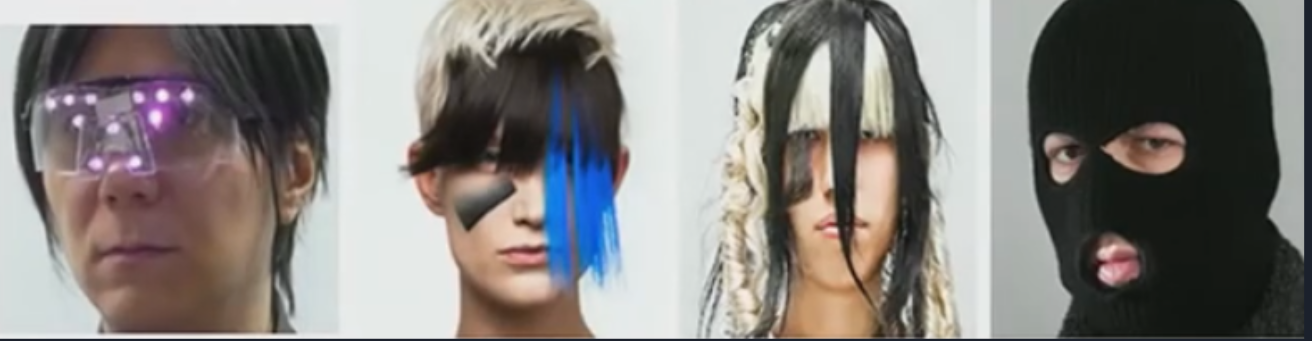
\includegraphics[width=0.8\textwidth]{Images/attacks.png}
\caption[]{Attacks that arouse suspicion\footnotemark[5]}
\end{figure}


\subsection{Generating adversarial noise}

In recent years Deep Neural Network models consisting of convolutional layers achieved state of the art performance in image recognition task [4]. Although their expressiveness is the cause of success, they also learn incomprehensible properties that are  counter-intuitive. Such incomprehensible properties were described by Szegedy et al. in \textit{Intriguing properties of neural networks} paper in 2014 [9]. Szegedy et al. surprised the machine learning community by finding that DNNs can be misled by slightly distorted input data. Szegedy et al. shown that it is possible to cause the network to categorize the image incorrectly using some barely noticeable disturbance that can be found by maximizing network prediction error. Under white-box scenario such disturbance can be found systemically in a similar way we find weights that minimizes prediction error - by using Gradient Descent algorithm. 

We can formalize the problem of finding perturbation $r$, as an optimization problem with 2 goals. First goal is misclassification, for a given $x$ find perturbation $r$ such that distance between DNN output $f(x+r)$ and some target class $h_t$ will be minimised. Second goal is imperceptibility of perturbation $r$, we achieve it by minimizing the norm of $r$. In other words, find a smallest perturbation $r$ that will cause specific misclassification $c_t$. . The objective of finding the perturbation is modeled by: 

\begin{equation}
\operatorname{argmin}_{r}\left(\left|f(x+r)-h_{t}\right|+\kappa|r|\right)
\end{equation}


Where classification function $f$ (in our case DNN) produces a probability distribution over $N$ classes (represented by a vector of size $Nx1$) where each element is $[0,1]$. $h_t$ is the one hot vector  of class $c_t$. $|\cdot|$ is norm function (e.g Norm 2). $\kappa$ a constant that can be tuned to balance the misclassification and imperceptibility objectives. If $f(\cdot)$ and $|\cdot|$ are differentiable, this optimization can be solved via simple optimization method like Gradient Descent. In our case $f(\cdot)$ is DNN, so we can be sure it is differentiable (without that property it would not be possible to train the neural network using back propagation). The usually used norm $|\cdot|$ is $Norm_2^2$, which is also differentiable. Optimal parameter $r$ can by fund using one of the modern machine learning frameworks like  Tensorflow or PyTorch. Example perturbation $r$ (amplified by 10 times to better visualize the change) and original image plus perturbation $x+r$ on Figure 12.  


\subsection{Impersonation and Dogging softmaxloss score}

In order to measure the correctness of classification authors used \textit{softmaxloss} score. For a given input $x$ of class $c_x$ (which one hot representation is $h_{c_x}$) that is classified as $f(x)$ (a vector of probabilities size $Nx1$), \textit{softmaxloss} is defined as:
Softmaxloss
\begin{equation}
\textit {softmaxloss}\left(f(x), c_{x}\right)=-\log \left(\frac{e^{\left\langle h_{c_{x}}, f(x)\right\rangle}}{\sum_{c=1}^{N} e^{\left\langle h_{c}, f(x)\right\rangle}}\right)
\end{equation}

Where $\langle\cdot, \cdot\rangle$ denotes inner product between two vectors. N is number of classes, $h_c$ is one hot representation of class $c$. \textit{Softmaxloss} is lower when classification $f(x)$ is correct, and higher when classification $f(x)$ is incorrect. \textit{Softmaxloss} can be used to measure effectiveness of Impersonation or Dodging  for a given perturbation $r$. 

\textbf{Impersonation}

When an attacker plans to impersonate a concrete target $t$, he / she needs to find such perturbation $r$ that will maximize probability of class $c_t$ for a classifier $f(x+r)$. We can define it as an optimization problem:

\begin{equation}
\operatorname{argmin}_{r} \textit{softmaxloss}\left(f(x+r), c_{t}\right)
\end{equation}

In other words, find perturbation $r$ such that will minimize distance between prediction $f(x+r)$ and target class $c_t$
\newpage

\textbf{Dodging}


In Dodging attacks, (in contrast to Impersonation) instead of impersonating concrete target $t$ attacker only goal is to not be recognised as himself / herself. This can be obtained by finding such perturbation $r$ that will minimize probability of recognising input $x$ as class $c_x$, or in other words by maximizing the value of $\textit{softmaxloss}(f(x+r), c_x)$. We can define it as an optimization problem:

\begin{equation}
\operatorname{argmin}_{r}\left(-\operatorname{softmaxloss}\left(f(x+r), c_{x}\right)\right)
\end{equation}


\subsection{Generating eye-glass frames}

As we shown in previous paragraph it is possible to find such perturbation  $r$ that will cause specific misclassification. Unfortunately using that method we change both face and background (See Figure 12). In initial assumptions we assumed that \textit{attacker can change only his/her appearance, but can’t change a background} (\textbf{Physical Realizability}), so we need to do something about it. 


The simple and efficient solution can be limiting perturbation to only the pixels that cover the face. It can be obtained by first performing image segmentation to find a face in an image and then limiting changes only to those pixels (See Figure 13). 

\begin{figure}[ht]
\centering
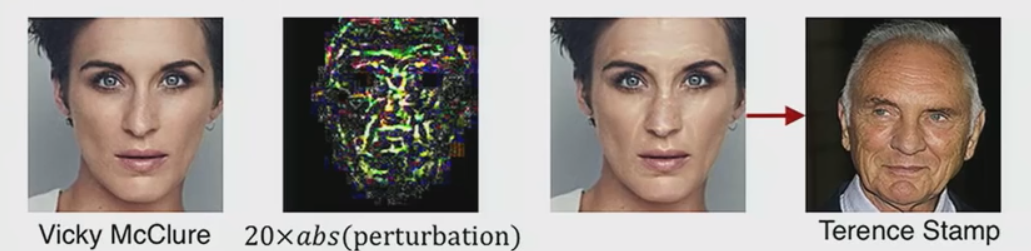
\includegraphics[width=0.8\textwidth]{Images/changes-applied-to-face-only.png}
\caption[]{Changes applied only to face not to background\footnotemark[5]}
\end{figure}

However, this approach does not solve all problems. First of all, founded face perturbations are small (in order to see them they have to be amplified 20 times See Figure 13) so it is very complicated to realize such perturbation in a real world. Second of all, cameras used in FRS have some physical limitations. Camera sampling errors are bigger than needed perturbations so carrying out such an attack would not be physically possible (attack would  actually not be detected by a camera).


For this reason, instead of changing the whole face, the authors of the paper came up with the idea of using facial accessories, specifically the eyeglass frames. The eyeglass frames are both physically realizable via 3d or even 2d printing technologies and inconspicuous - they don't arouse that much suspicion. The eyeglass frames perturbation can be generated in a similar way as face perturbation. First we perform image segmentation in order to find eyes in the image and then limiting perturbation $r$ only to the pixels around eyes in the shape of frames (See Figure 14). 

\begin{figure}[ht]
\centering
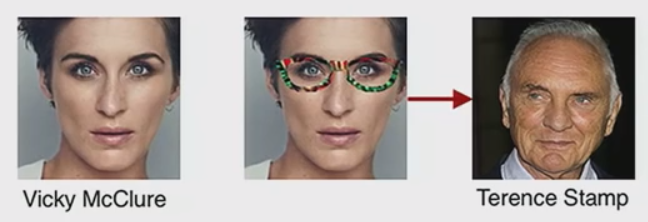
\includegraphics[width=0.8\textwidth]{Images/eyeglasses-attack.png}
\caption[]{Eyeglass attack\footnotemark[5]}
\end{figure}